\documentclass[a4paper,twoside]{article}

\usepackage{epsfig}
\usepackage{subfigure}
\usepackage{calc}
\usepackage{amssymb}
\usepackage{amstext}
\usepackage{amsmath}
\usepackage{amsthm}
\usepackage{multicol}
\usepackage{pslatex}
\usepackage{apalike}
\usepackage{SCITEPRESS}     % Please add other packages that you may need BEFORE the SCITEPRESS.sty package.

\usepackage{url}% http://ctan.org/pkg/url
\usepackage{flushend}

\subfigtopskip=0pt
\subfigcapskip=0pt
\subfigbottomskip=0pt

\begin{document}


\title{Enabling GPU Virtualization in Cloud Environments}
\author{\authorname{Sergio Iserte, Francisco J. Clemente-Castell\'o, Adri\'an Castell\'o,\\Rafael Mayo and Enrique S. Quintana-Ort\'i}
\affiliation{Department of Computer Science and Engineering\\Universitat Jaume I - Castell\'o de la Plana, Spain}
\email{\{siserte, fclement, adcastel, mayo, quintana\}@uji.es}}

\keywords{Cloud Computing, GPU Virtualization, AWS, Resource Management}

\abstract{The use of accelerators, such as graphics processing units (GPUs), to reduce the execution time of compute-intensive applications has become more popular during the past few years. 
These devices increment the computational power of a node thanks to its parallel architecture.
This trend has led cloud vendors, as Amazon Web Services, or middlewares such as OpenStack to add to their current facilities   
instances of virtual machines including GPUs. 
To fullfil these needs, the guest hosts must be equipped with GPUs which will be barely utilized if a non GPU-enabled Virtual Machine is running in the host.
The solution presented in this work is based on GPU virtualization and shareability in order to reach an equilibrium between service supply and applications' demand of accelerators. 
Hence, we propose to decouple real GPUs from the nodes by using the virtualization technology rCUDA. 
With this software configuration, GPUs can be accessed from any VM avoiding the need  
of having a physical GPUs in the guest host. 
Moreover, we study the viability of this approach by using a public cloud 
service configuration and develop a module for OpenStack middleware in order to 
add support for the virtualized devices and the logic to manage them. 
The results demonstrate this is a viable configuration which adds flexibility to the current and well-known 
cloud solutions. 
}

\onecolumn \maketitle \normalsize \vfill

\section{\uppercase{Introduction}}
\label{sec:introduction}
Nowadays, many cloud vendors have started offering virtual machines (VMs) with GPUs in order to provide
GPGPU computation services to users. A few relevant examples include 
Amazon Web Services (AWS)\footnote{\url{https://aws.amazon.com}}, 
Penguin Computing\footnote{\url{http://www.penguincomputing.com}}, 
Softlayer\footnote{\url{http://www.softlayer.com}} and 
Microsoft Azure\footnote{\url{https://azure.microsoft.com}}.
In the public scope, one of the most popular cloud vendors is AWS, that offers a wide range of preconfigured instances ready to be launched.
Alternatively, owning the propper infrastructure, a private cloud can be deployed using a specific middleware such as
Openstack\footnote{\url{https://www.openstack.org}} or Opennebula\footnote{\url{http://opennebula.org}}.

Unfortunately, sharing GPU resources among multiple VMs in cloud environments 
is not straightforward as is in a physical servers resulting into a low utilization rate.
On one hand, instances in public clouds are not easily customizable. 
On the other, in a private cloud, although the instances can be customized in many aspects, when referring to GPUs
the number of options is reduced.
Moreover, neither vendors nor tools are offer GPGPU wasting the opportunity of providing flexibility and boosty the utilization of GPU resources in both private or public clouds.

These devices were adopted with the release of the CUDA programming model for
NVIDIA GPUs~\cite{cuda65}, which includes both high- and low-level application programming interfaces (APIs)
to allow the use of NVIDIA devices as general-purpose
accelerators.
Following CUDA, OpenCL~\cite{opencl} appeared as an attempt
to offer a cross-vendor solution.

The current approach to assemble a cluster with accelerators consist in installing 
one or more of these devices in each compute node.
However, these configurations often present a low
utilization rate of the computational resources
 because of mismatches between the application's type of parallelism
and the accelerators' architecture.

Remote virtualization has been recently proposed to deal with the low-usage problem 
(e.g. {rCUDA}~\cite{tonithesis},
DS-CUDA~\cite{dscuda}, gVirtus~\cite{gvirtus}, vCUDA~\cite{vcuda}, VOCL~\cite{vocl}, and SnuCL~\cite{snucl}).

Roughtly speaking these virtualization frameworks 
enable cluster configurations with fewer GPUs than nodes.  The goal is that 
GPU-equipped nodes act as GPGPU (general-purpose GPU) servers, yielding a CUDA-sharing solution that potentially achieves
a higher overall GPU load in the system.

The main goals of this work are to study current cloud solutions from 
the point of view of HPC field and GPU usage, and to analyze and improve 
them by adding flexibility with GPU virtualization. In order to reach 
this goal, we select rCUDA, a virtualization tool that is possibly the more complete 
and up-to-date for NVIDIA GPUs.

The rest of the paper is structured as follows. 
In Section~\ref{sec:background} the technologies we introduce used in this work;
Section~\ref{sec:state} summarizes previous work in this field; 
Section~\ref{sec:motivation} states the motivation to carry out this work;
the effort to use AWS is explained in Section~\ref{sec:workingaws};
while the work with Openstack is described in Section~\ref{sec:gpgpuOS};
finally Section~\ref{sec:conclusions} summarizes the advances and Section~\ref{sec:future} proposes the next steps
 of this research.

\section{\uppercase{Background}}
\label{sec:background}
\subsection{The rCUDA Framework}
\label{sec:rcuda}
{rCUDA}~\cite{toniparco} is a middleware that enables transparent access
to any NVIDIA GPU device present in a cluster from all compute
nodes. The GPUs can be accessed and shared between nodes, and a single node can use all the graphic accelerators
as if they were local.
These features focus in attaining higher accelerator utilization rates in the overall system while simultaneously reducing
resource, space, and energy requirements~\cite{energy14}.
rCUDA is structured following a client-server distributed
architecture: the client middleware runs in the same cluster node where the application demanding GPGPU
acceleration services is executed, providing a transparent replacement for the
native CUDA libraries. Furthermore, the server middleware is executed in the
cluster nodes from which the actual GPUs provide the requested GPGPU service.
To support a concurrent scenario where GPUs are shared between
processes\slash nodes, {rCUDA} manages separate device contexts for
each client application.

The {rCUDA} 5.0 client exposes the same interface as the regular NVIDIA
CUDA 6.5 release~\cite{cuda65}, including the runtime and driver
APIs as well as other commonly used libraries such as cuBLAS, cuFFT, cuSparse or cuRand.
Therefore, applications are not aware of the fact that they are being executed
on top of a virtualization layer.
To deal with new GPU programming models, {rCUDA} has been recently extended to accommodate 
directive-based models such as OmpSS~\cite{repara15} and OpenACC~\cite{cluster15}.

The integration of remote GPGPU virtualization with global
resource schedulers such as SLURM~\cite{sbacpad14} completes this powerful
technology, making accelerator-enabled clusters more flexible and
energy-efficient.

\subsection{Amazon Web Services}
\label{sec:aws}
AWS~\cite{aws} is a public cloud computing provider, 
composed of several services, such as 
 cloud-based computation, storage and other functionality, 
that enables organizations and/or individuals to deploy
services and applications on an on-demand basis. 
These services replace local IT infrastructure for companies and provide agility and instant elasticity matching 
perfectly with their software requirements.

From the point of view of HPC, AWS offers high performance facilities via 
instances equipped with GPUs and high performance network interconnection, which 
are common resources leveraged in this research field.

\subsection{OpenStack}
\label{sec:openstack}

OpenStack~\cite{OpenStack} is a cloud operating system that provides Infrastructure as a Service (IaaS). 
It is able to control large pools of compute, storage, and networking resources throughout a 
datacenter. All these resources are managed through a dashboard or an API that gives administrators 
control while empowering their users to provision resources through a web interface
or a command-line interface.  
OpenStack supports most available hypervisors and handles provisioning 
and life-cycle management of VMs.
 
The OpenStack architecture offers flexibility to create a custom cloud, with no proprietary hardware
or software requirements and the ability to integrate with legacy systems and third party technologies. 

From the HPC perspective, OpenStack offers high performance configurations using
multiple supported hypervisors and different hardware architectures. Despite in OpenStack is possible to 
specify some extra parameters requesting special resources, like GPUs, choosing a host based on the existence
of a GPU is currently unsupported~\cite{OpenStackGPU}. 

\section{\uppercase{State-of-the-Art}}
\label{sec:state}
Our solutions to the defficiency exposed in the previous section is based on GPU virtualization, sharing resources in order
to attain a fair balance between supply and demand. 
While several efforst with the same goal have been made in the past, as exposed next, 
none of them is so ambitious as ours. 

The work in~\cite{younge2013enabling} allows the VM managed
by the hypervisor Xen to access the GPUs in the physical
node, with the implied limitations that a node cannot 
use more GPUs than those hosted in the machine, and idle GPUs can not be shared with other machines. The solution presented 
by gVirtus~\cite{giunta2010gpgpu} virtualizes GPUs and makes
them accessible for any VM in the cluster. However, this kind
of virtualization strongly depends on the hypervisor and, so
does its performance. Another similar solution is presented in gCloud~\cite{diab2013dynamic}. 
iWhile this solution is not yet integrated in a Cloud Computing Manager, its main
drawback is that the code of the applications must be modified
in order to be run in the virtual-GPU environment. A runtime component to provide abstraction
and sharing of GPUs is presented in~\cite{becchi2012virtual}, which allows scheduling policies 
to isolate and share GPUs in a cluster for a set of applications. 
The work introduced in~\cite{jungpgpu} is more mature, however,
it is only focussed on compute-intensive HPC applications. 

Our proposal goes further and, in addition to 
bringing solutions for all kind of HPC applications, it is aimed
to boost flexibility in the use of GPUs.

\section{\uppercase{Motivation}}
\label{sec:motivation}

Cloud computing and storage have gained wide appeal  
during the last years thanks to the easy set up 
process and the low IT invest. The services offered in the cloud are useful for companies and individuals 
that look for temporary access to the last technology without spending a 
huge amount of money. In general, the systems provided by cloud 
companies match with the those requested thanks to its flexibility.

Two different kinds of cloud approaches are currently available:
on one hand, public facilities, such as AWS or 
Microsoft Azure that allow users to chose a pre-configured system.   
On the other hand, institutions/companies 
are able to deploy their own cloud infrastructure by a software as OpenStack.  

In both cases, the power of current cloud facilities relies on the use 
of VMs which  
emulate a physical node with its own 
CPUs, storage, network interconnection, GPU and operating system (OS). 
However, providing a VM equipped with a GPU implies
that the guest host must be equipped with at least one GPU, and
once it has been assigned to an instance, no other VM can use
it. Therefore, the number of VMs that are allowed to use GPUs is 
limited by the number of the installed devices. This lack of 
flexibility is also present in the cluster configurations, where 
depending on the users' necessities, 
two approaches to introduce GPGPU computation can be identified:
the conservative option, features a lot of hosts with GPUs to 
ensure that is likely to satisfy all requests; in a
more daring approach, a reduced count of some GPU-enabled nodes is available, in the hope that a large burst of GPU requests 
 does not exhaust the cluster's resources.

The use of a virtualization technology such as {rCUDA} adds 
the desired flexibility because this software detaches the GPUs 
from the nodes where they are installed, allowing all nodes in a cluster
not only to use them as if they were local, but also to share them 
achieving a higher utilization rate and reducing the idle periods.
Thanks to the ``shareability'' introduced by {rCUDA}, all VMs in the cloud 
environment can leverage and share all GPUs installed in 
the physical nodes, removing past limitations. 

Our work focuses on AWS as a public 
solution, and on OpenStack software as a private cloud environment. 
In order to achieve our goal, these cloud facilities need to be provided with the {rCUDA} software. In addition, for OpenStack, a module for managing virtualized GPUs 
needs to be implemented.  



\section{\uppercase{GPGPU share service with AWS}}
\label{sec:workingaws}
In this section, we briefly expose the current user-level features 
provided by AWS and then analyze this service  
from the point of view of the GPU usage. 
Next, we describe the scenarios and experiments where virtualized GPUs are utilized and show a number of first results.

\subsection{Current Features}
This subsection identifies the most common features checked during 
the VM's creation step.

\subsubsection{Instances}

An instance is a pre-configured VM focused on an 
specific target. Among the large list of instances offered by AWS, 
we can find cases for general purpose (T2, M4 and M3); computer science optimized 
(C4 and C3); memory optimized (R3); storage optimized (I2 and D2) and 
GPU capable (G2). Each type of instance has its own purpose cost (price). 
Moreover, each instance offers a different number of CPUs as well as network 
interconnection which can be: low, medium, high or 10Gb.

For our study, we worked in the AWS availability zone US EAST (N. VIRGINIA). 
The instances available in that zone presented the features shown in the Table~\ref{table:awsInstances}. 

\begin{table}[htb]
\renewcommand{\arraystretch}{1.3}
\caption{Shown HPC instances available in US EAST (N. VIRGINIA) in June 2015.}
\label{table:awsInstances}
\tabcolsep=0.09cm
\begin{center}\begin{tabular}{cccccc}
Name & vCPUs & Memory & Network & GPUs & Price\\ \hline \hline
c3.2xlarge & 8 & 15 GiB & High & 0 & \$ 0.21\\ \hline
c3.8xlarge & 32 & 60 GiB & 10 Gb & 0 & \$ 1.68 \\ \hline
g2.2xlarge & 8 & 15 GiB & High & 1 & \$ 0.65\\ \hline
g2.8xlarge & 32 & 60 GiB & 10 Gb & 4 & \$ 2.6 \\ \hline
\end{tabular}\end{center}\end{table}

For the following experiments, we select C3 family instances, which are not equipped with GPUs, as clients; whereas instances of the G2 family will act as servers.   

\subsubsection{Networking}
Table~\ref{table:awsInstances} shows that each instance integrates a different 
network. Thus, taking into account that bandwidth 
is critical when GPU virtualization is applied, a simple test to verify the 
real network bandwidth is needed.

\begin{table}[htb]
\renewcommand{\arraystretch}{1.3}
\caption{IPERF results between selected instances.}
\label{table:iperf}
\tabcolsep=0.24cm
\begin{center}\begin{tabular}{cccc}
Server & Client & Network & Bandwidth\\ \hline \hline
g2.8xlarge & c3.2xlarge & High & 1  Gb/s\\ \hline
g2.8xlarge & c3.8xlarge & 10Gb & 7.5  Gb/s\\ \hline
g2.8xlarge & g2.2xlarge & High & 1 Gb/s\\ \hline
g2.8xlarge & g2.8xlarge & 10Gb & 7.5  Gb/s\\ \hline
\end{tabular}\end{center}\end{table}

To evaluate the actual bandwidth, we executed 
the IPERF\footnote{\url{http://iperf.fr/}} tool between the instances explained in 
the Table~\ref{table:awsInstances} with the results shown in the Table~\ref{table:iperf}.
From this experiment, we can assume that the nomenclature ``High'' corresponds to a 1~Gb interconnection network and the 10~Gb has 
a real bandwidth of 7.5~Gb/s.
Moreover, it looks like the instances equipped with a ``High'' interconnection network
are constrained by software to 1~Gb/s since the theoretical and real bandwidth 
match perfectly. The real gap between sustantiable and theoretical bandwidth can be observed with 
the 10~Gb interconnection, which reaches up to 7.5~Gb/s.


\subsubsection{GPUs}
An instance relies on a VM that runs on a real node with its own virtualized components. 
Therefore it is possible that AWS uses a virtualization framework to offer GPU services to all the instances.
Although, the {\tt nvidia-smi} command indicates that the GPUs installed are NVIDIA GRID K520, 
we need to verify that they are non-virtualized devices. For this proposal, we execute the NVIDIA SDK test {\tt bandwidthtest}. 
As shown in the Table~\ref{table:bwt}, the bandwidth achieved in this test is higher than the network bandwith, revealing that the accelerator is an ad-hoc GPU. 
% \begin{table}[htb]
% \renewcommand{\arraystretch}{1.3}
% \caption{NVIDIA SDK {\tt bandwidthtest} execution transferring 32MB using pageable memory using local GPU.}
% \label{table:bwt}
% \tabcolsep=0.09cm
% \begin{center}\begin{tabular}{cccc}
% Name &  Data Movement & Network & Bandwidth \\ \hline \hline
% g2.2xlarge & Host to Device & High& 3,004 MB/s \\ \hline
% g2.2xlarge & Device to Host & High& 2,809 MB/s\\ \hline
% g2.8xlarge & Host to Device & 10 Gb& 2,814 MB/s\\ \hline
% g2.8xlarge & Device to Host & 10 Gb& 3,182 MB/s\\ \hline
% \end{tabular}\end{center}\end{table}

\begin{table}[htb]
\renewcommand{\arraystretch}{1.3}
\caption{NVIDIA SDK {\tt bandwidthtest} execution transferring 32MB using pageable memory in local GPU.}
\label{table:bwt}
\tabcolsep=0.09cm
\begin{center}\begin{tabular}{ccc}
Name &  Data Movement & Bandwidth \\ \hline \hline
g2.2xlarge & Host to Device & 3,004 MB/s \\ \hline
g2.2xlarge & Device to Host & 2,809 MB/s\\ \hline
g2.8xlarge & Host to Device & 2,814 MB/s\\ \hline
g2.8xlarge & Device to Host & 3,182 MB/s\\ \hline
\end{tabular}\end{center}\end{table}

\subsection{Testbed Scenarios}
In this section, we introduce the different client-server configurations. 
All scenarios are based on the maximum number of instances 
that a user can freely select without submitting a formal request. 
In particular, the maximum number for ``g2.2xlarge'' is 5 and for ``g2.8xlarge'' it is 2.

All the instances deployed operate the RHEL 7.1 64-bit OS and version 6.5 of CUDA. 
We design three configuration scenarios for our tests:

\begin{itemize}
\item Scenario A (Figure~\ref{subfig:aws1}) shows the most common 
 hardware configuration in clusters, with each node  
populated with one GPU. Here, a simple node can access to 5 GPUs 
using the ``High'' network. 

\item Scenario B (Figure~\ref{subfig:aws2}) is composed by 2 server nodes equipped 
with 4 GPUs each one, and a GPU-less client. This scenario includes 
a 10Gb network, and the client can execute the application using up to 8 GPUs.

\item Scenario C (Figure~\ref{subfig:aws3}) combines scenarios A and B. A 
single client, using a 1Gb network interconnection, can leverage 13 GPUs as if they were local.
\end{itemize}

\begin{figure*}[ht]
\centering
\subfigure[5 remote GPUs over 1GbE.]{%
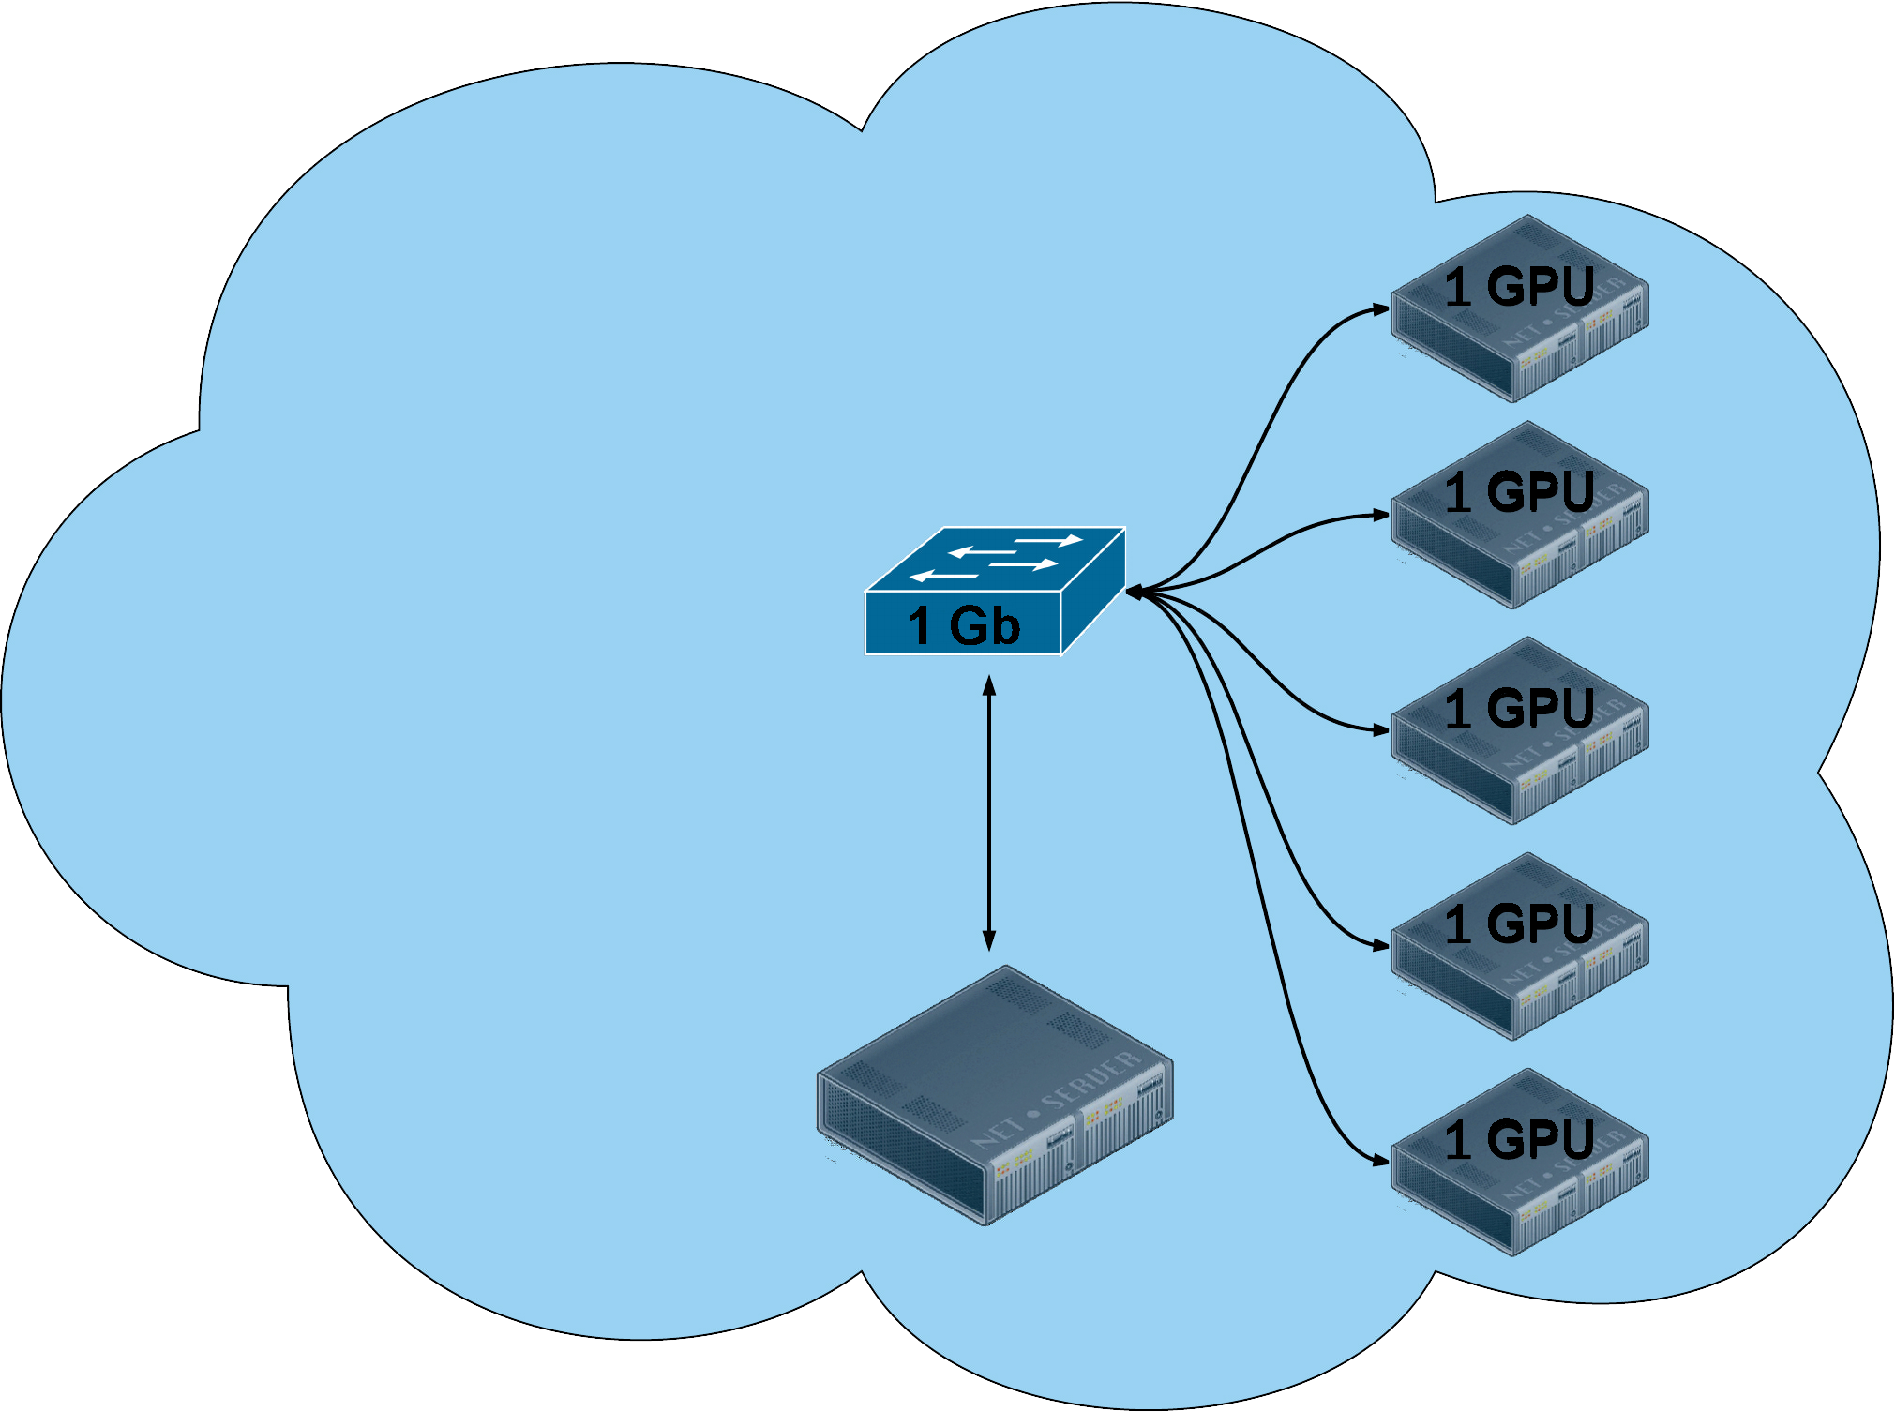
\includegraphics[width=0.315\linewidth]{images/aws3.pdf}
\label{subfig:aws1}}
\quad
\subfigure[8 remote GPUs over 10GbE.]{%
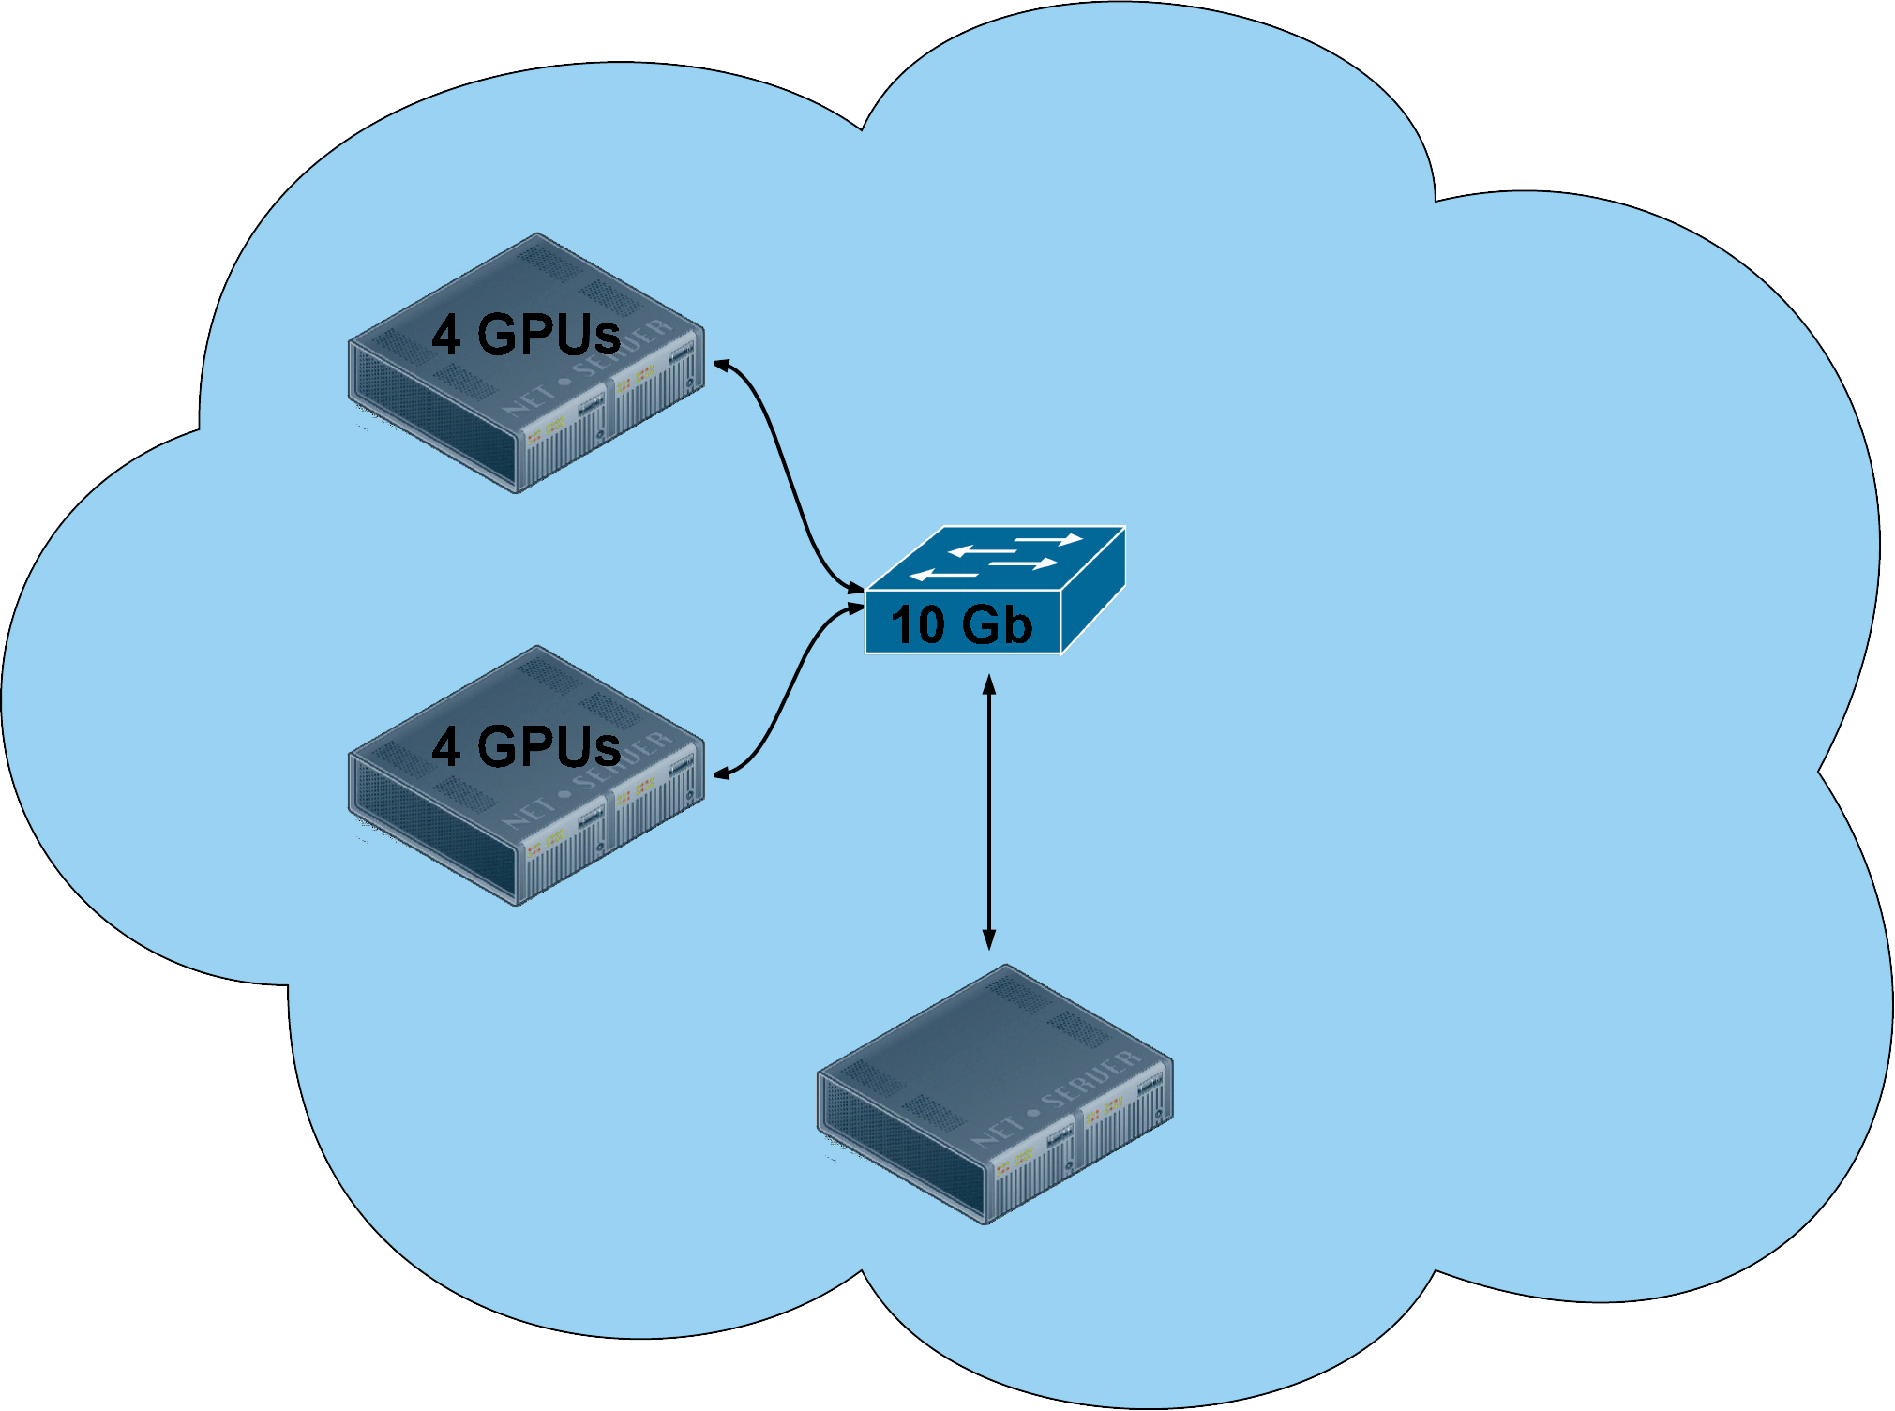
\includegraphics[width=0.315\linewidth]{images/aws2.pdf}
\label{subfig:aws2}}
\subfigure[13 remote GPUs over 1GbE.]{%
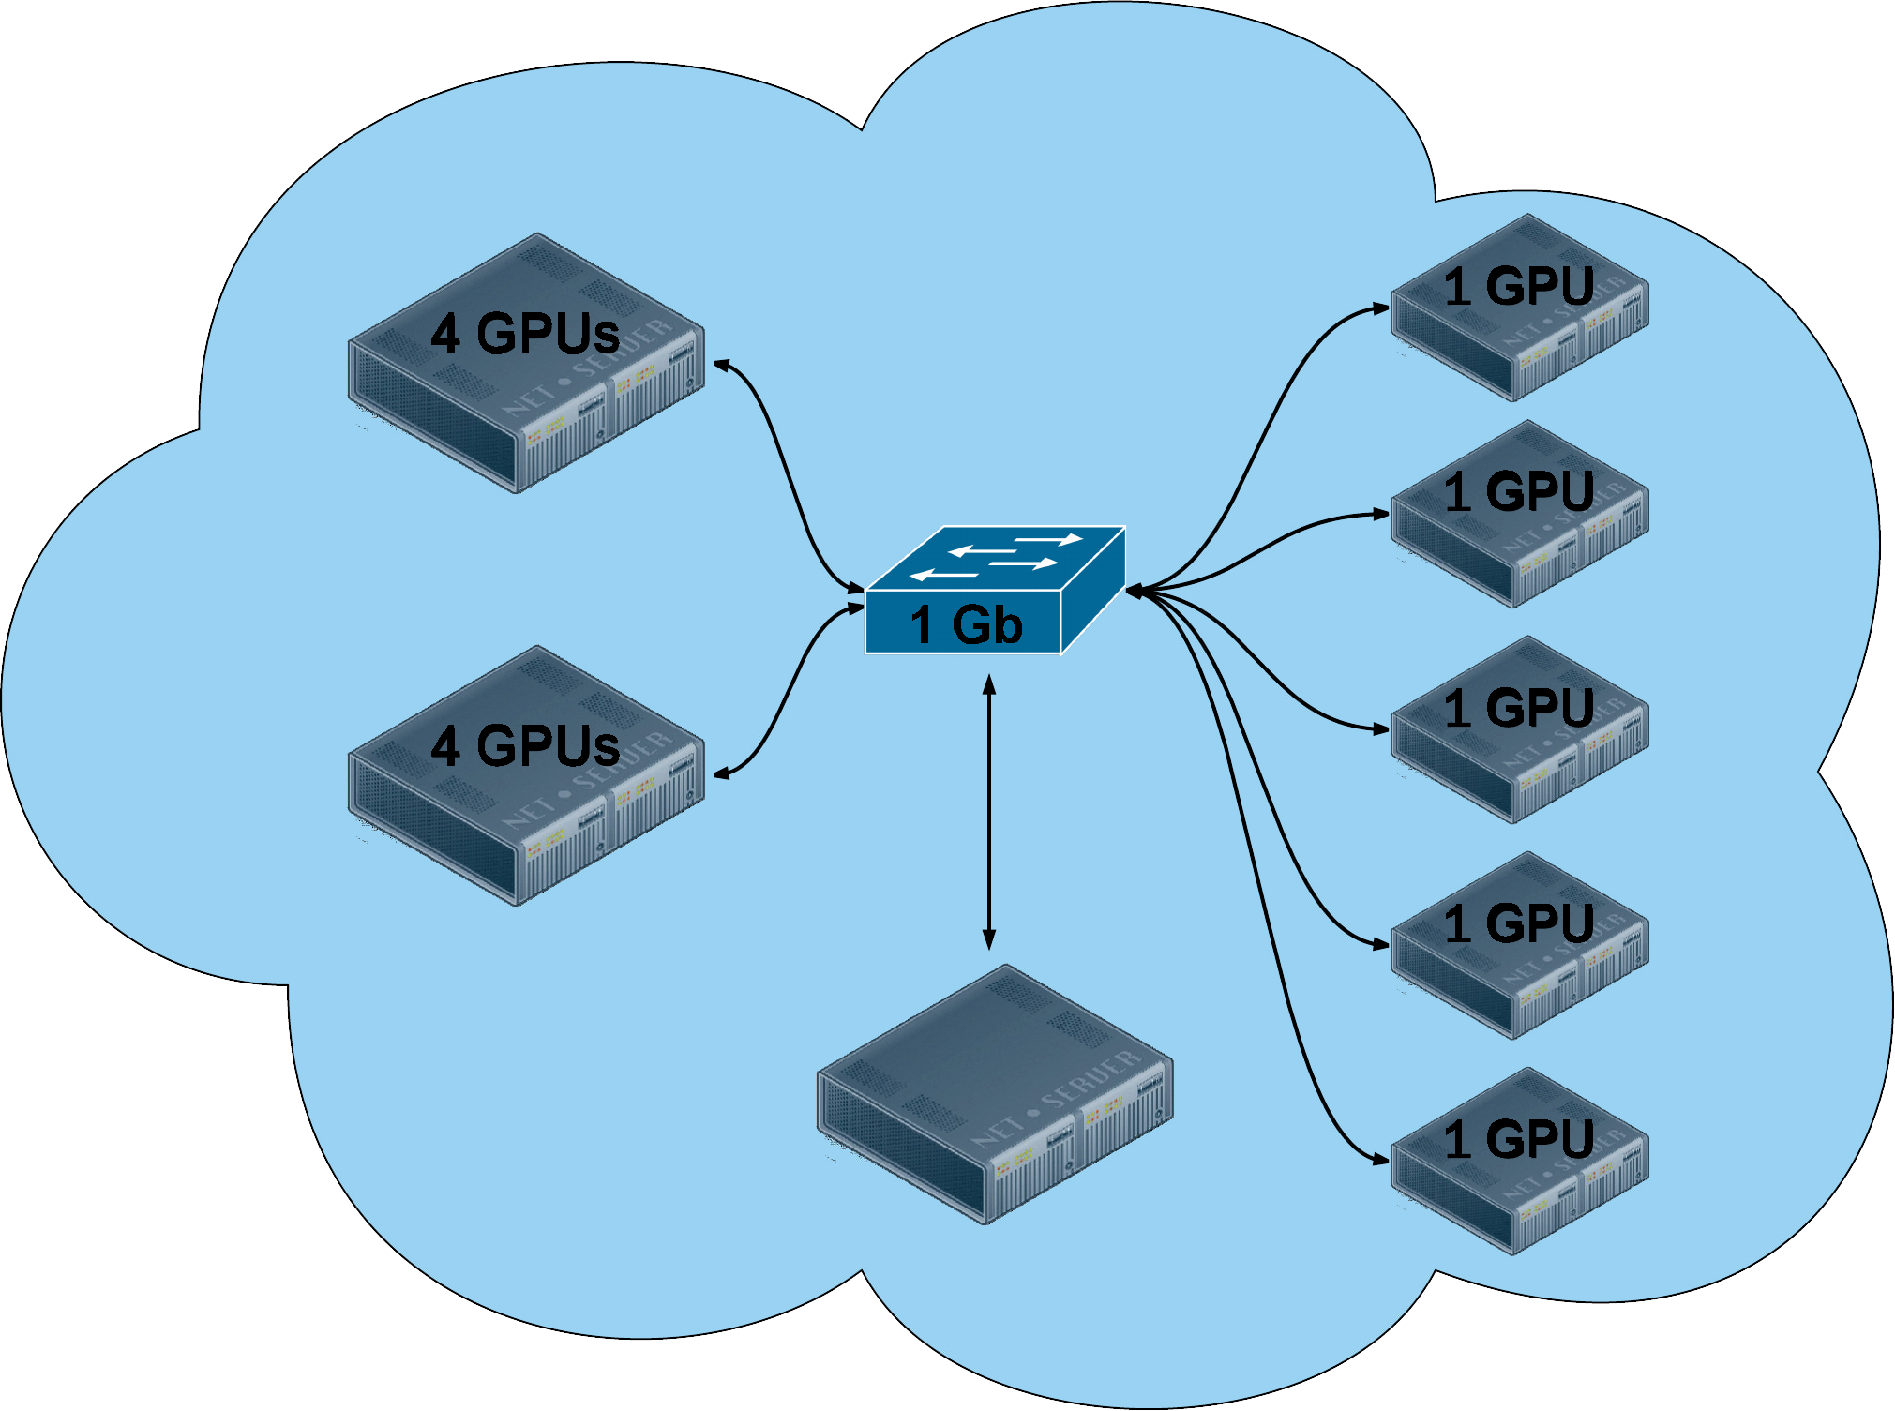
\includegraphics[width=0.315\linewidth]{images/aws1.pdf}
\label{subfig:aws3}}
\caption{Configurations where an AWS instance, acting as a client, employs several remote GPUs.}
\label{fig:aws}
\end{figure*}

Once the scenarios are configured from the point of view of hardware, 
the {rCUDA} middleware needs to be installed in order to add 
the required flexibility to the system. The {rCUDA} server is 
executed in the server nodes and the {rCUDA} libraries are invoked from the node that acts as client.

In order to evaluate the network bandwidth using a remote GPU, we re-applied NVIDIA SDK {\tt bandwidthtest}.
Table~\ref{table:bwtrcuda} exposes that the bandwidth is limited by the network.

\begin{table}[htb]
\renewcommand{\arraystretch}{1.3}
\caption{NVIDIA SDK {\tt bandwidthtest} execution transferring 32 MB using pageable memory using {rCUDA}.}
\label{table:bwtrcuda}
\tabcolsep=0.09cm
\begin{center}\begin{tabular}{cccc}
Scenario &  Data Movement & Network & Bandwidth \\ \hline \hline
A & Host-to-Device & High& 127 MB/s \\ \hline
A & Device-to-Host & High& 126 MB/s\\ \hline
B & Host-to-Device & 10 Gb& 858 MB/s\\ \hline
B & Device-to-Host & 10 Gb& 843 MB/s\\ \hline
\end{tabular}\end{center}\end{table}

\subsection{Experimental results}
In this subsection we employ two GPU applications to assess the benefits of GPU virtualization.

The first application is {\tt MonteCarloMultiGPU}, from the NVIDIA SDK, a code that is compute bound (its execution barely involves memory operations). 
This was launched with the default configuration, ``scaling=weak'', which adjusts the size of the problem depending on the number of accelerators.
Figure~\ref{fig:mont-opt} depicts the options per second calculated by the application running on the scenarios in Figure~\ref{fig:aws} as well as using local GPUs. 
For clarity, we have removed the results observed for Scenario B as they are exactly the same as those obtained from Scenario C with up to 8 GPUs. 
In this particular case, rCUDA (remote GPUs) outperforms CUDA (local GPUs) because the former loads the libraries when the daemon is started~\cite{tonithesis}.
With rCUDA we can observe differences in the results between both scenarios. 
Here, Scenario A can increase the throughput because the GPUs do not share the PCI bus with other devices as each node only is equipped with one GPU.
On the other hand, when the 4-GPU instances (``g2.8xlarge'') are added (Scenario C), the PCI bus constrains the communication bandwidth, hurting the scalability.

\begin{figure}[htb]
  \centering
  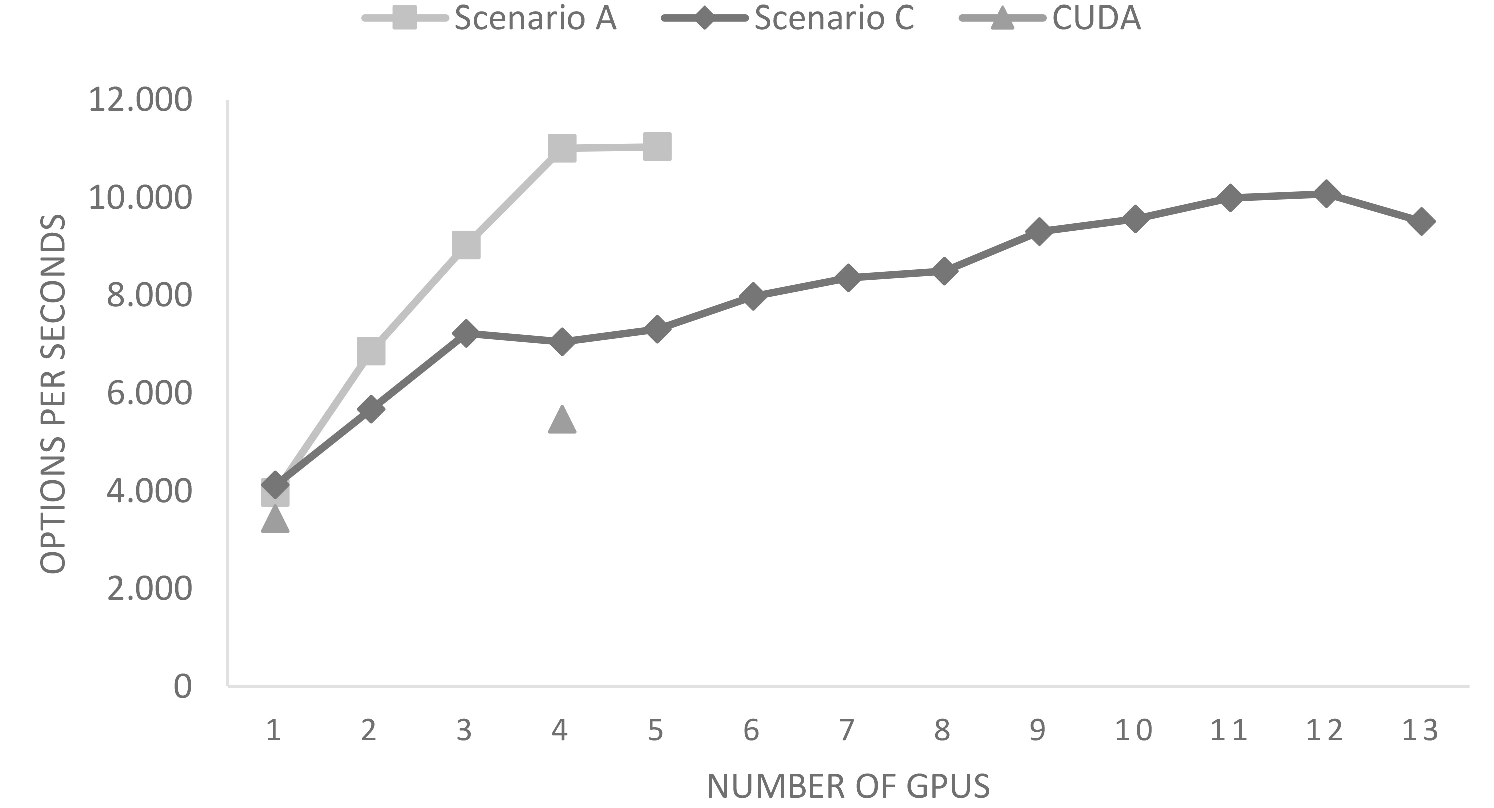
\includegraphics[width=\linewidth]{images/mont.pdf}
  \caption{NVIDIA SDK {\tt MonteCarloMultiGPU} execution using local (CUDA) and remote (Scenarios A and C) GPUs.}
  \label{fig:mont-opt}
\end{figure}

The second application, LAMMPS\footnote{\url{http://lammps.sandia.gov}}, 
is a classical molecular dynamics simulator that can be applied at the atomic, 
meso, or continuum scale. 
From the implementation perspective, this multi-process application employs 
at least one GPU to host its processes, but can benefit from the presence of multiple GPUs.
Figure~\ref{subfig:lammps1} shows that, for this application, the use of remote GPUs 
does not offer any advantage over the original CUDA. 
Furthermore, for the execution on remote GPUs, the difference between both networks is small, although, the results observed with the ``High'' network are worse than those obtained with the ``10 Gb'' network.
In execution of LAMMPS on a larger problem (see Figure~\ref{subfig:lammps2}), CUDA still performs better, but the interesting point is the execution time when using remote GPUs. 
These are almost the same even with different networks, which indicates that the transfers turn the interconnection network into a bottleneck. 
For this type of application, enlarging the problem size compensates the negative effect of a slower network.

\begin{figure}[htb]
\centering
\subfigure[Run size = 100.]{%
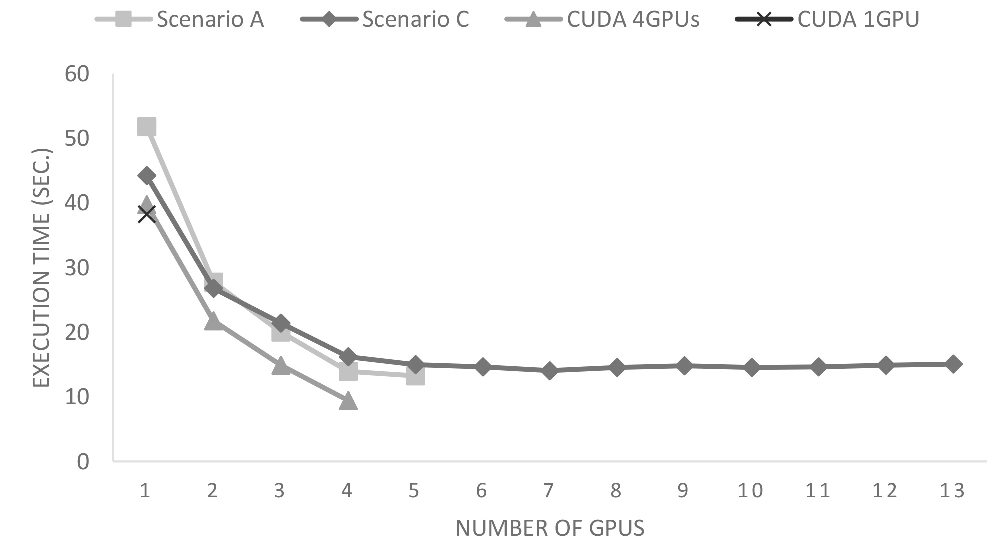
\includegraphics[width=\linewidth]{images/lammps1.pdf}
\label{subfig:lammps1}}
\quad
\subfigure[Run size = 2000.]{%
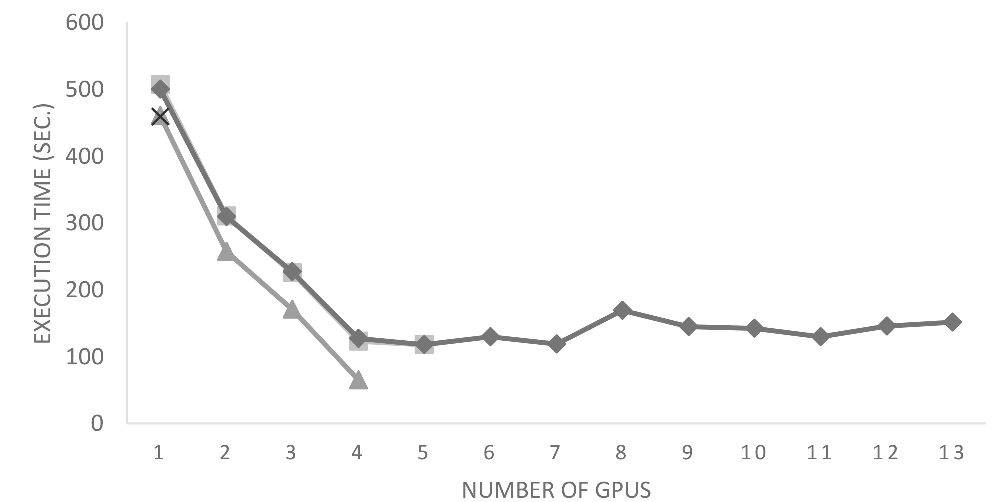
\includegraphics[width=\linewidth]{images/lammps2.pdf}
\label{subfig:lammps2}}
\caption{Execution time of LAMMPS.}
\label{fig:lammps}
\end{figure}

\subsection{Discussion}
The previous experiments reveal that the AWS GPU-instances are not appropriate for HPC
because neither the network nor the accelerators are powerful enough to deliver high performance
when running compute-intensive parallel applications. 
In other words, AWS is more oriented toward offering a general-purpose service than to provide high performance.
Also, AWS fails in offering flexibility as it forces the user to choose between a basic instance with a GPU and a powerful instance with 4 GPUs.

Table~\ref{table:awsInstances} shows that the resources of the ``g2.8xlarge'' are quadrupled, but so is the cost per hour.
Therefore, in the case of having other necessities (in terms of the instances type), using GPU virtualization technology we could in principle attach an accelerator to any type of instance.
Furthermore, reducing the budget spent in cloud services is possible by customizing the resources of the available instances.
For example, we can work on an instance with 2 GPUs for only \$ 1.3 by launching 2 ``g2.2xlarge'' and using remote GPUs, avoiding to pay the double for features that we do not need in ``g2.8xlarge''.

The last conclusion is related to GPU-shareability. 
As we deduced, AWS reserves GPU-capable physical machines which will be idle until a GPU-instance request is made.
Maintaining an expensive accelerator in a standby state is counter-productive. 
It makes more sense to dedicate less devices, accessible from any machine.

\section{\uppercase{GPGPU Shared Service in OpenStack}}
\label{sec:gpgpuOS}
In this section we describe our work on OpenStack, from the development of an external module to handle remote GPUs to the physical setup and its validation.

\subsection{Managing remote GPUs with OpenStack}
The main idea is to evolve from the original OpenStack architecture (see Figure~\ref{subfig:os-orig})
 to a solution where a new shared service, responsible for the GPU accelerators, becomes integrated into the architecture (see Figure~\ref{subfig:os-mod}).
This new service brings more flexibility when managing GPUs and new working modes for GPGPU computation in the Cloud.
As illustrated in Figure~\ref{fig:internal}, we alter the original OpenStack Dashboard with a new parser, 
which splits the HTTP query in order to make use of both the GPGPU API for GPU-related operations, and the Nova API for the rest of the computations. 
The new GPGPU Service grants access to GPUs in a VM, but also allows the creation of ``GPU-pools'', consisting of a set of independent GPUs (logically disattached from the nodes) that can be assigned to one or more VMs.

\begin{figure}[htb]
  \centering
  \subfigure[Version Icehouse]{
    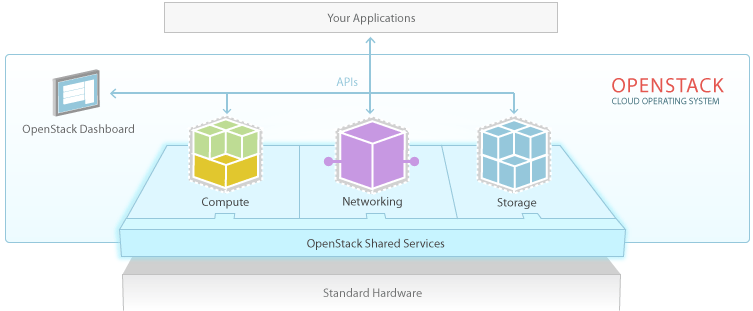
\includegraphics[width=\linewidth]{images/os-orig.png}
    \label{subfig:os-orig}
   }
   \quad
  \subfigure[With GPGPU module]{
    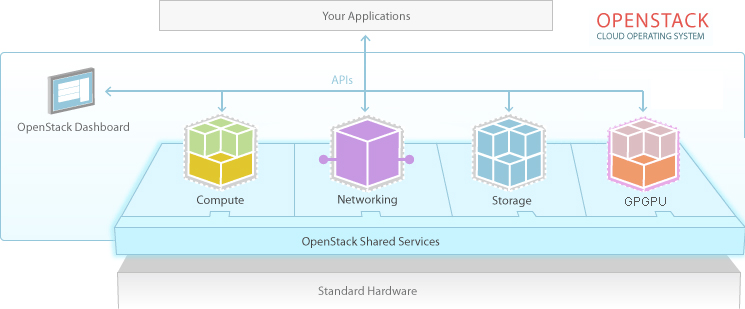
\includegraphics[width=\linewidth]{images/os1.jpg}
    \label{subfig:os-mod}
   }
  \caption{OpenStack Architecture.}
  \label{fig:os}
\end{figure}

\begin{figure}[htb]
  \centering
  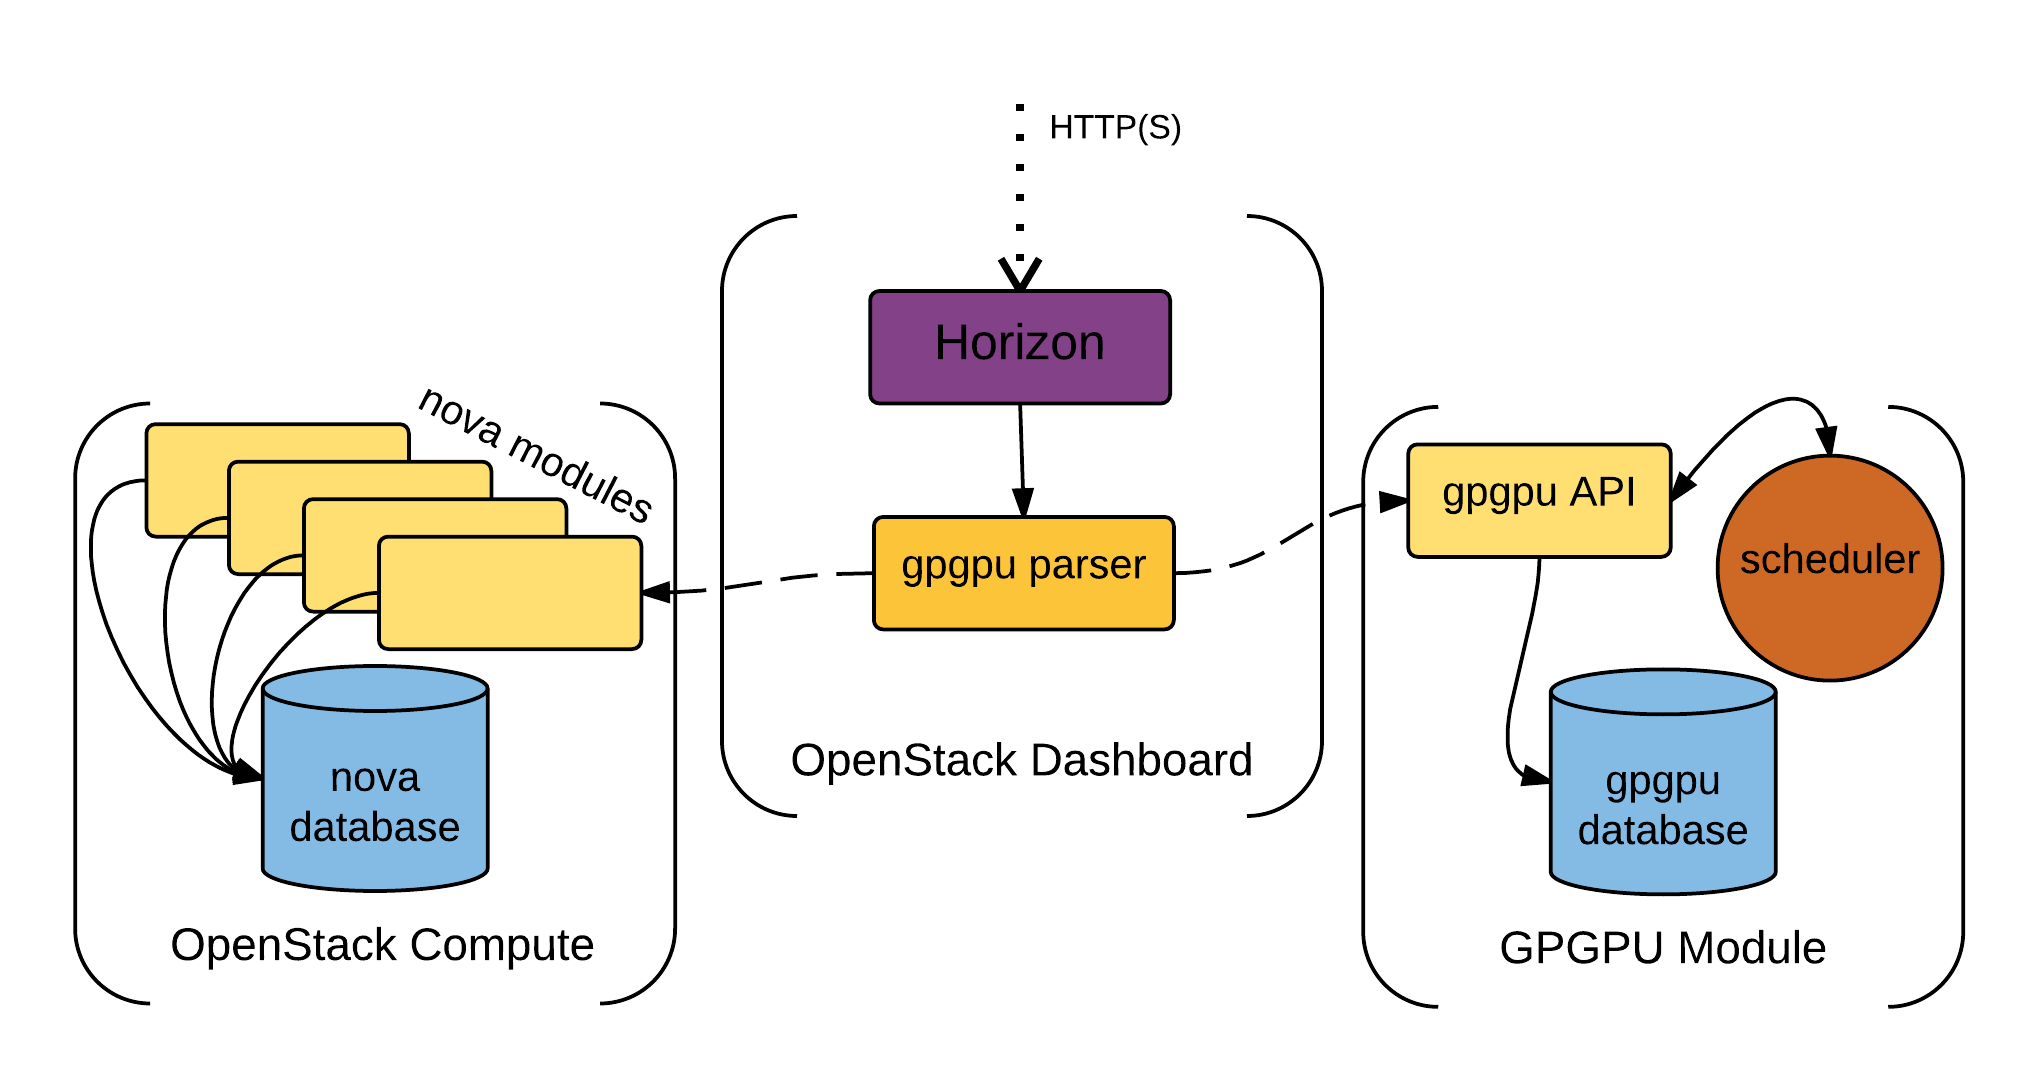
\includegraphics[width=\linewidth]{images/os2.png}
  \caption{Internal Communication among modules.}
  \label{fig:internal}
\end{figure}

Thanks to the modular approach of the GPGPU Service, the Nova Project does not need to be modified, and the tool can be easily ported to other Cloud Computing solutions.

\subsection{Working Modes}
The developed module allows users to set up any of the scenarios displayed in Figure~\ref{fig2}. 
The users are given two configuration options to decide whether a physical GPU will be completely reserved for an instance (first column) or the instance will address a partition of the GPU as if it were a real device (second column).
We refer to this as the ``mode'', with possible values being: ``exclusive'' or ``shared''. 
Let us assume there are 4 GPU devices in the cluster (independently of where they were hosted). 
An example of these scenarios is shown in Figure~\ref{fig2}.
There, in the ``exclusive'' mode the instance monopolizes all the GPUs; while in the ``shared'' mode, the GPUs are partitioned. 
As a result of sharing the GPU memory, the instance will be able to work with up to 8 GPUs, provided that each partition can be addressed as an independent GPU.

Moreover, the users are also responsible for deciding whether a GPU (or a pool) will be assigned to other instances. 
This behaviour is refereed as ``scope'', and it determines that a group of instances is logically connected to a pool of GPUs.
Working with the ``public'' scope (bottom row of Figure~\ref{fig2}) implies that the GPUs of a pool can be used simultaneously by all the instances linked to it.
Again, the GPU pool can be composed of ``exclusive'' or ``shared'' GPUs.

\begin{figure}[htb]
  \centering
  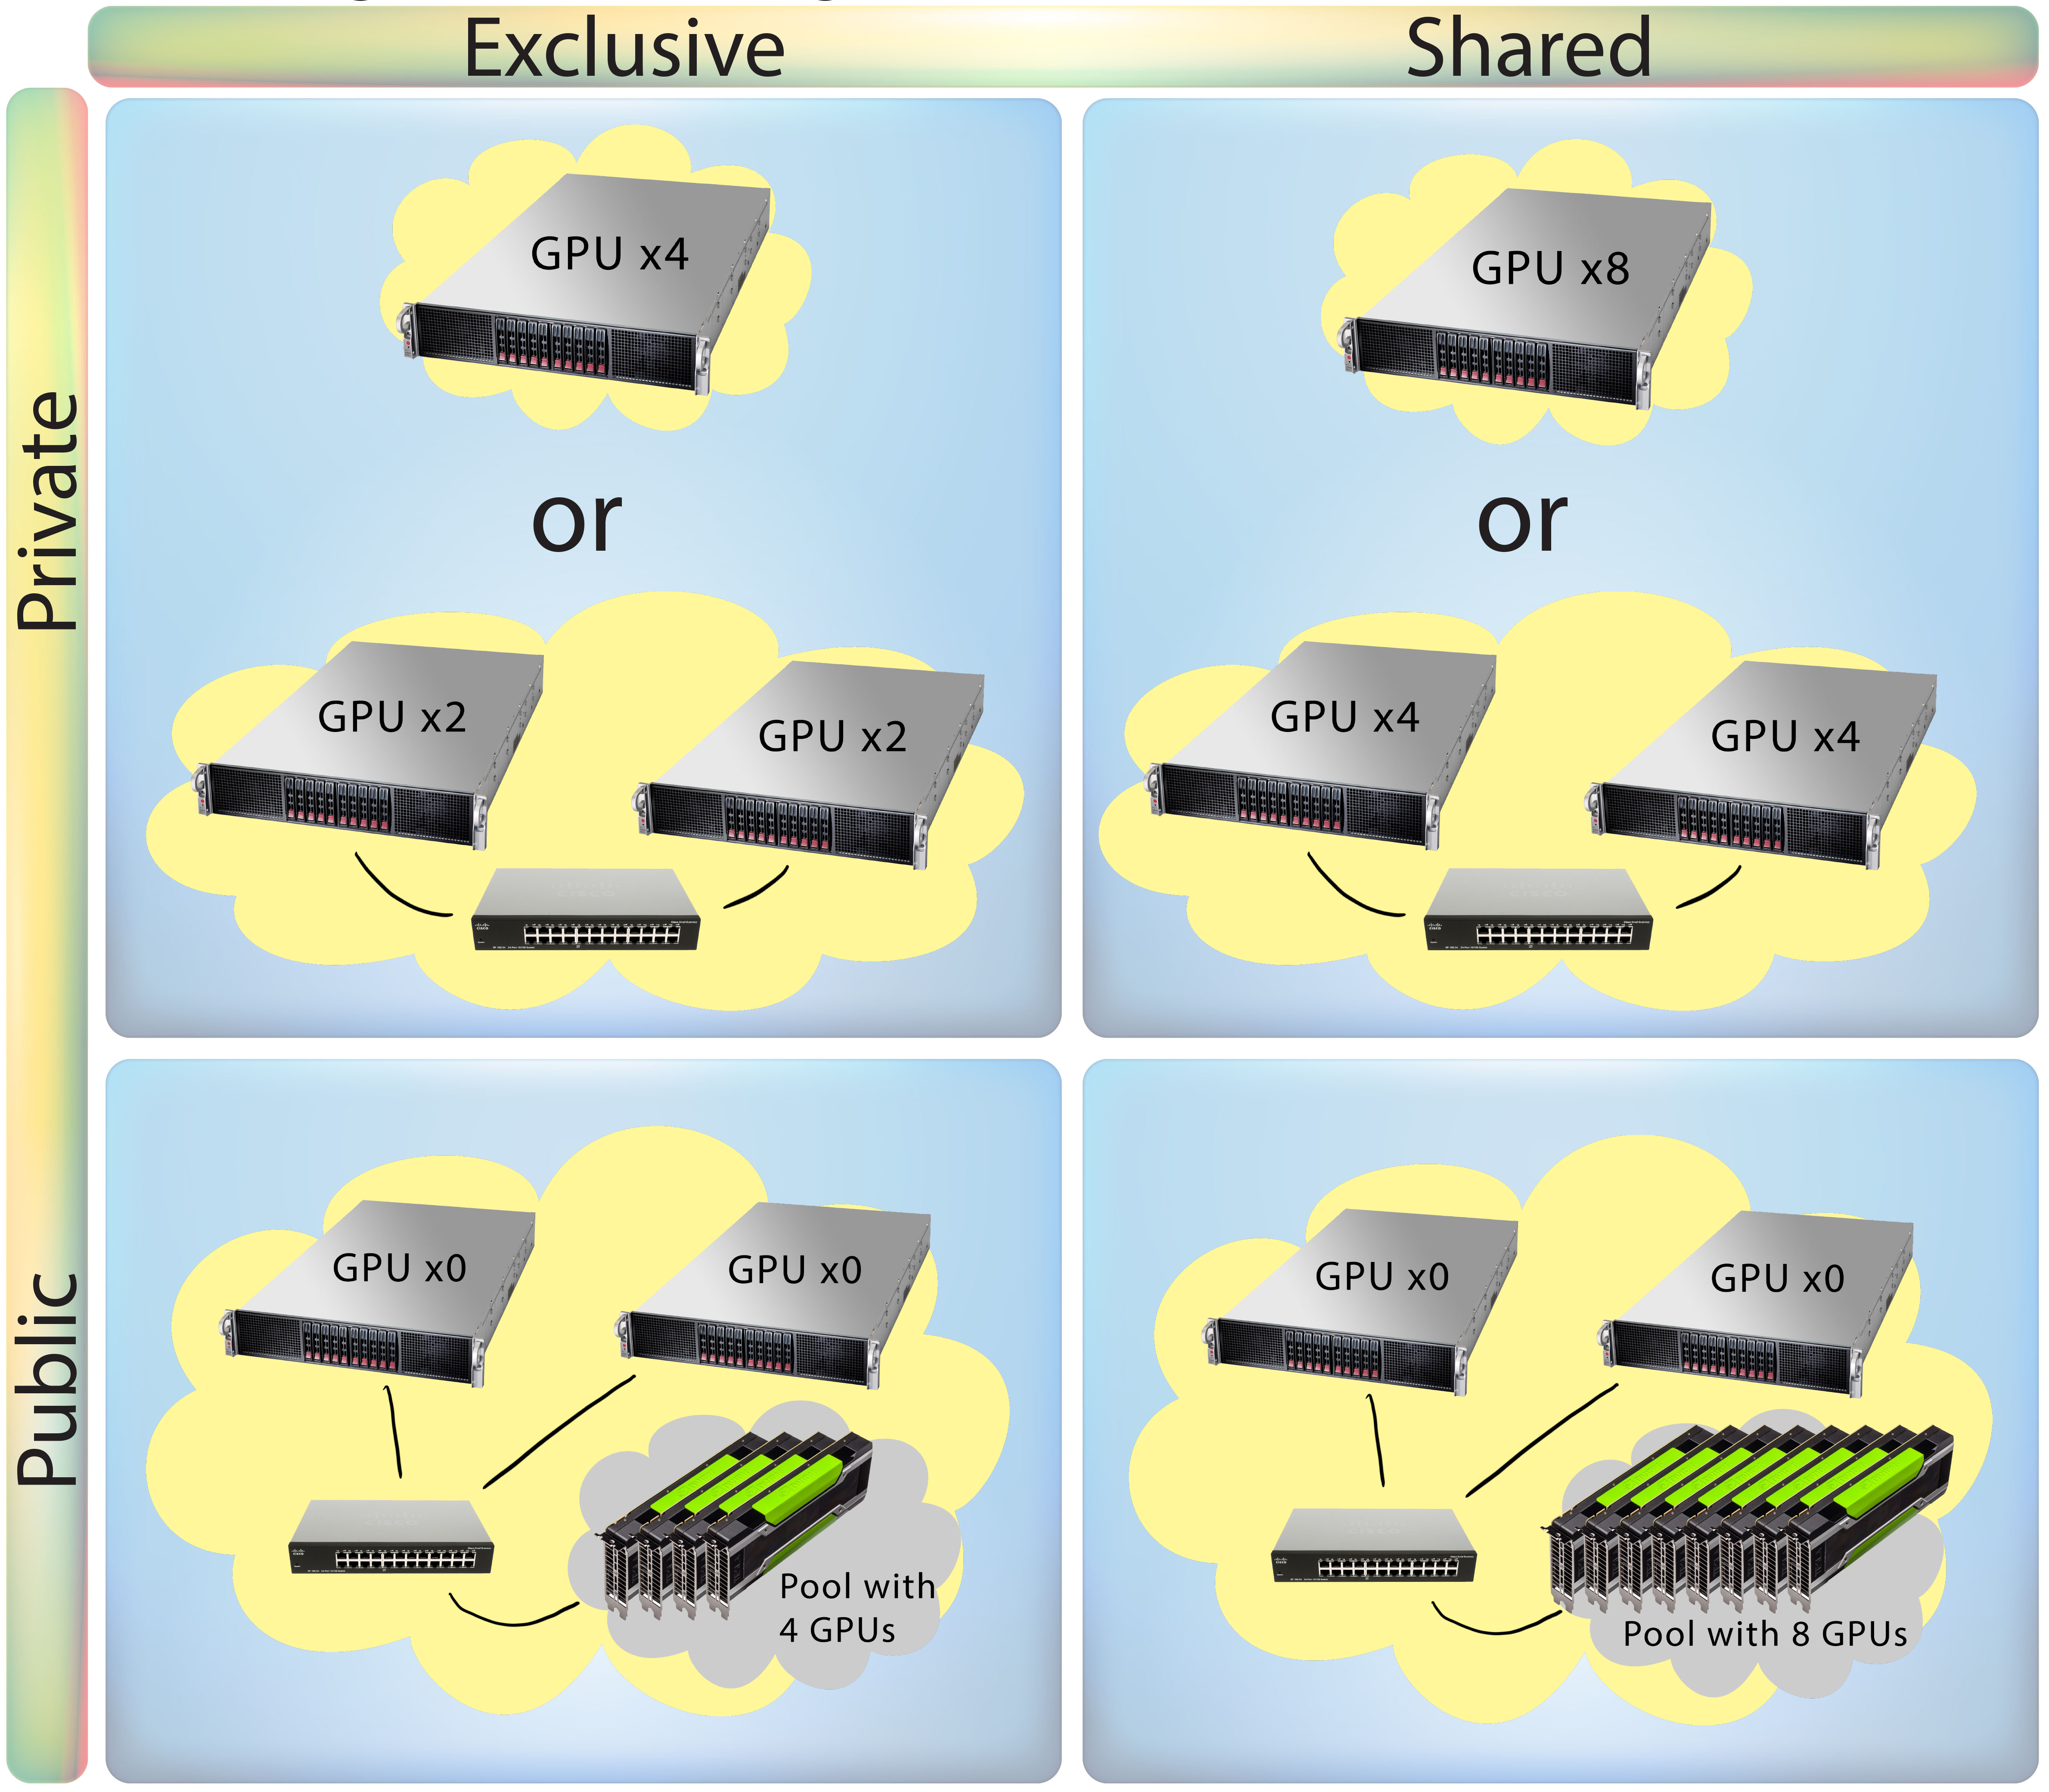
\includegraphics[width=.5\textwidth]{images/workingmodes.jpg}
  \caption{Examples of working modes.}
  \label{fig2}
\end{figure}

\subsection{User Interface}
In order to deal with the new features, several modifications have been planned in the OpenStack Dashboard, they have not been implemented yet, though.
First of all, the Instance Launch Panel should be extended with a new field, where the user could assign an existing GPU pool, create a new one, or keep the instance without accelerators of this kind.
When the option ``New GPU Pool'' is chosen, the proper fields for the pool configuration would appear (see Figure~\ref{fig:ui-launch}).
Furthermore, a new panel with the existent GPUs displays all the information related to GPUs (see Figure~\ref{fig:ui-rgpus}).

\begin{figure}[htb]
  \centering
  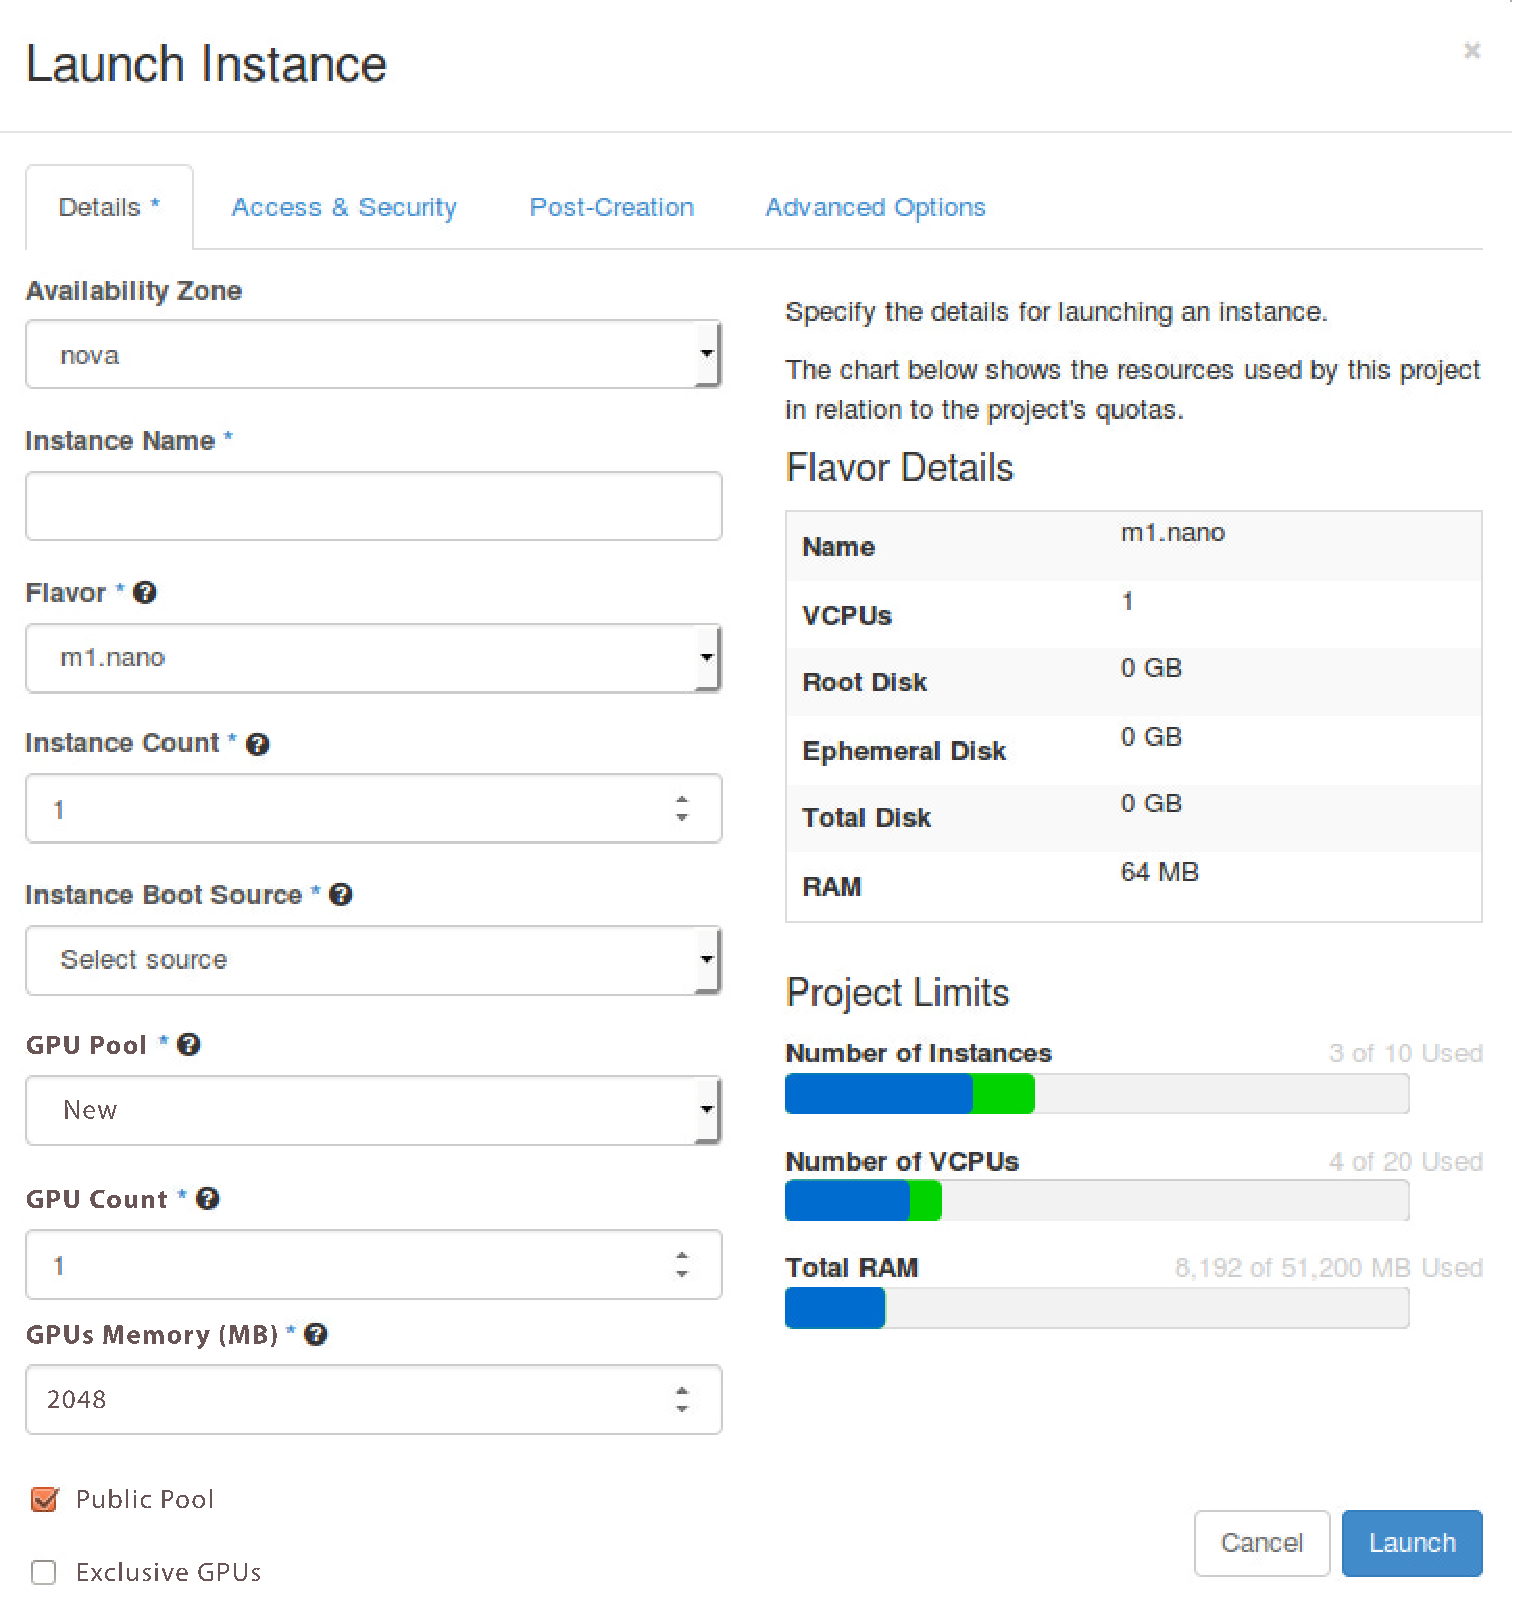
\includegraphics[width=\linewidth]{images/UI-launch.pdf}
  \caption{Launching Instances and assigning GPUs.}
  \label{fig:ui-launch}
\end{figure}
  
\begin{figure}[htb]
  \centering
  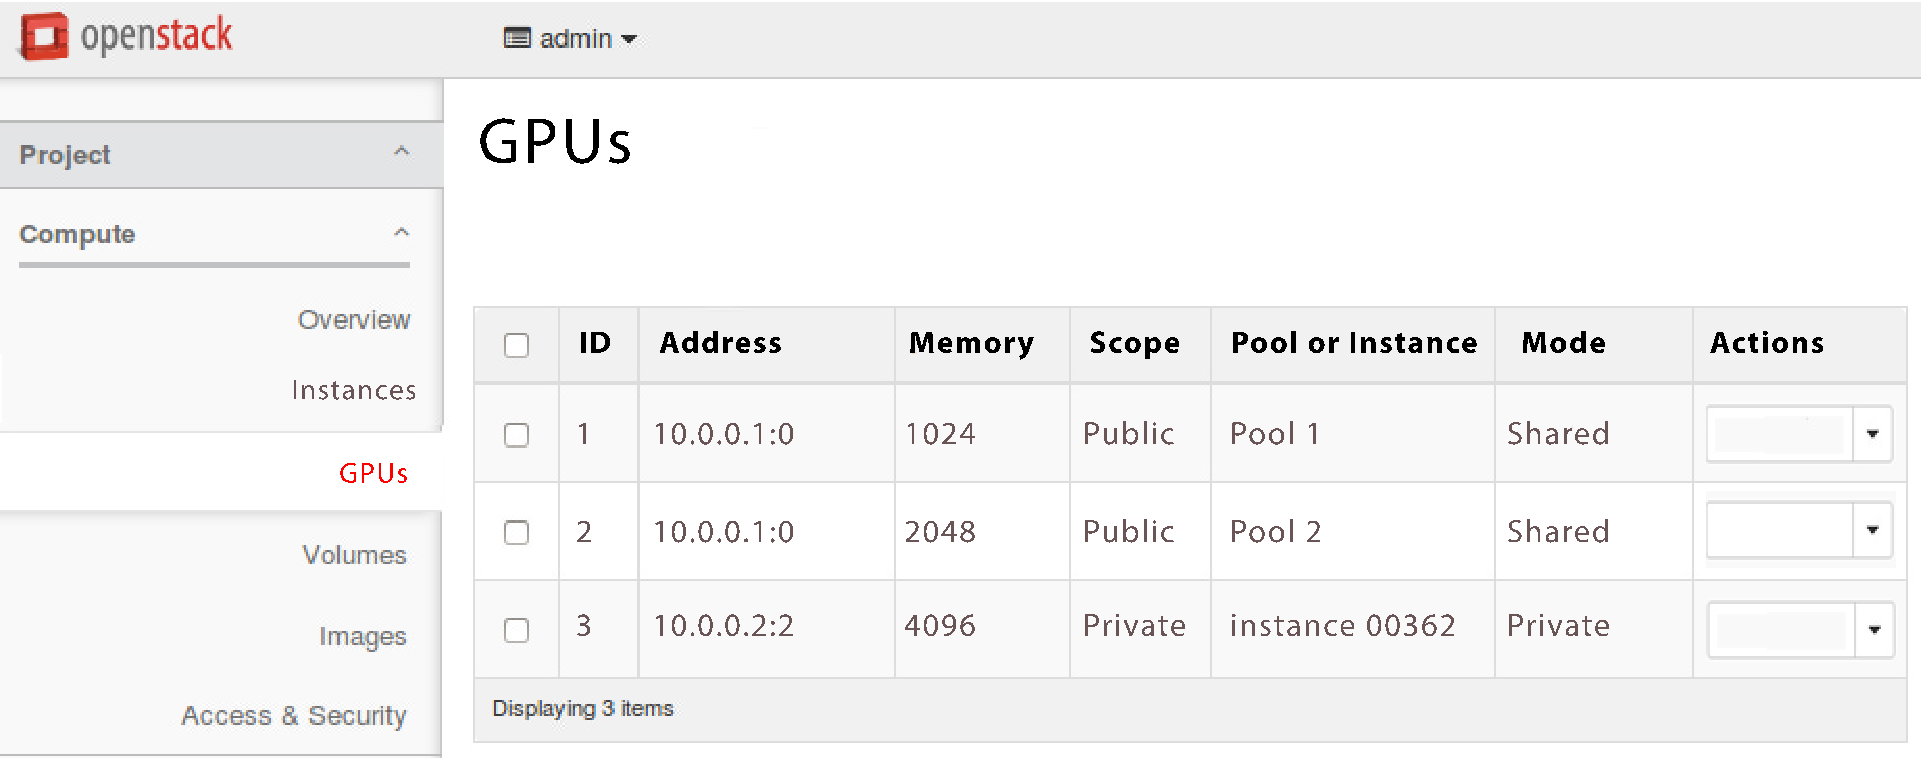
\includegraphics[width=\linewidth]{images/UI-rgpus.pdf}
  \caption{GPU Information Panel.}
  \label{fig:ui-rgpus}
\end{figure}

\subsection{Experimental Results}
The following tests were executed on 2 sets of nodes interconnected by a 1Gb Ethernet network.
All the nodes were equipped with an Intel Xeon E7420 quadcore processor, at 2.13 GHz, and 16 Gbytes of DDR2 RAM memory at 667 MHz.

The first set, in charge of providing the cloud environment,
consisted of 3 nodes.
To deploy an IaaS, we used OpenStack Icehouse version, and QEMU/KVM 0.12.1 as the hypervisor.
A fully-featured OpenStack deployment requires at least three nodes: a controller manages the compute nodes 
where the VMs are hosted; a network node manages the logic virtual network for the VMs, and one or more compute nodes run the hypervisor and VMs.

The second set, composed of 4 nodes, were auxiliary servers with a Tesla C1060 GPU each. 
The OS was a Centos 6.6; and the GPUs used CUDA 6.5. 
The GPU virtualization support was based on rCUDA v5.0. 

We have designed 6 different set-ups which can be divided into 2 groups: exclusive and shared GPUs. 
The exclusive mode provides, at most, 4 accelerators. 
The number of available GPU in “shared” mode will depend on the partition size. 
In this particular case, we halved the GPU memory, resulting 8 partitions that can be addressed as independent GPUs.
For each group, we deployed virtual clusters of 1, 2 and 3 nodes, where the application processes were executed. 
The instances were launched with the OpenStack predefined flavor “m1.medium”, which determines a configuration of VMs consisting of 2 cores and 4~GB of memory.

MCUDA-MEME~\cite{Liu2010} was the application selected to test the set-ups. 
Thus is an MPI software, where each process must have access to a GPU.
Therefore, the number of GPUs determines the maximum number of processes we can launch.

Figure~\ref{fig3} compares the execution time of the application with different configurations over different setups. 
We used up to 3 nodes to spread the processes and launched up to 8 processes (only 4 in exclusive mode), one per remote GPU.
We can first observe that the performance is higher with more than one node, because the traffic network is distributed among the nodes.
In addition, the shortest execution time is obtained by both modes (exclusive and shared) when running their maximum number of processes with more than one node.
This seems to imply that it is not worth to scale (increase) the number of resources, because the performance growth rate is barely increasing.
Although, the time is lower when the GPUs are shared, the setup cannot take advantage of an increase in the number of devices.

\begin{figure}[htb]
  \centering
  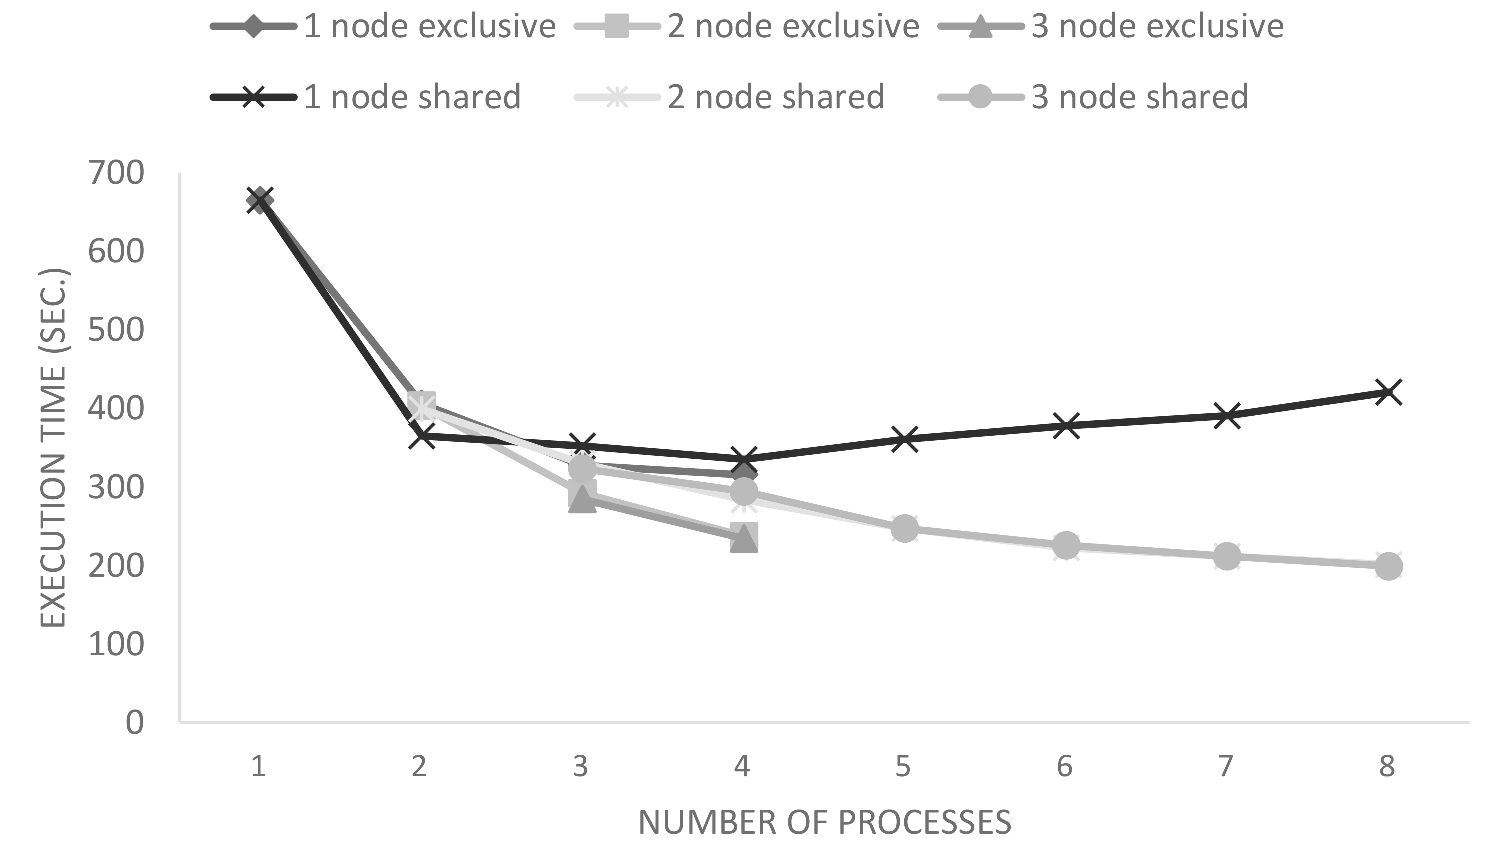
\includegraphics[width=\linewidth]{images/mcudameme-os.pdf}
  \caption{Scalability results of MCUDAMEME with a different number of MPI processes.}
  \label{fig3}
\end{figure}

\subsection{Discussion}
The network interconnect restricts the performance of our executions.
The analysis in~\cite{tonithesis} reveals that improving the network infrastructure can make a big different for GPU virtualization.

The most remarkable achievement is the wide range of possible configurations and the flexibility to adapt a system to fit the user requirements. 

In addition, with this virtualization technology, the requests for GPU devices can be fulfilled with small investment in infrastructure and maintenance.
Energy can be saved not only thanks to the remote access and the ability to emulate several GPUs using only a few real ones, but also by consolidating the accelerators in a single machine (when possible), or turning down nodes when their GPUs are idle. 

\section{\uppercase{Conclusions}}
\label{sec:conclusions}
We have presented a complete study of the possibilities offered by AWS when it comes to GPUs. 
The constraints imposed by this service motivated us to deploy our own private cloud, in order to gain flexibility when dealing with these accelerators.
For this purpose, we have introduced an extension of OpenStack which can be easily exploited to create GPU-instances as well as manage the physical GPUs to better profit from them.

As we expected, due to the limited bandwidth of the interconnects used in the experimentation, the performances observed for the GPU virtualized scenarios in the tests were quite low.
On the other hand, we have created new operation modes that open interesting new ways to leverage GPUs in situations where having access to a GPU is more important than having a powerful GPU to boost the performance.

\section{\uppercase{Future work}}
\label{sec:future}
The first item in the list of pending work is an upgrade of the network to an interconnect that is more prone to HPC.
In particular, porting the setup and the tests to an infrastructure with an Infiniband network will shed light on the viability of this kind of solutions for HPC.
Similar reasons, motivate us to try other Cloud vendors which better support for HPC.

Looking for real situations where performance is less important than flexibility will drive us to explore alternative tools to easily deploy GPU-programming computer labs.

Finally, an interesting future work is to design new strategies in order to decide where a remote GPUs is created and assigned to a physical device
Concretely, to innovate scheduling policies can enhance the flexibility offered by the GPGPU module for OpenStack.

\section*{\uppercase{Acknowledgements}}
The authors would like to thank the IT members of the department Gustavo Edo and Vicente Roca for their help.

This research was supported by Universitat Jaume I research project (P11B2013-21); and projects
TIN2014-53495-R from MINECO and FEDER.

\bibliographystyle{apalike}
{\small
\bibliography{paper}}


\end{document}
